
%(BEGIN_QUESTION)
% Copyright 2012, Tony R. Kuphaldt, released under the Creative Commons Attribution License (v 1.0)
% This means you may do almost anything with this work of mine, so long as you give me proper credit

Skygg området/-ene i dette diagrammet som representerer følgende integral (forutsatt at hver horisontale og vertikale inndeling i diagrammet har trinnverdi 1):

$$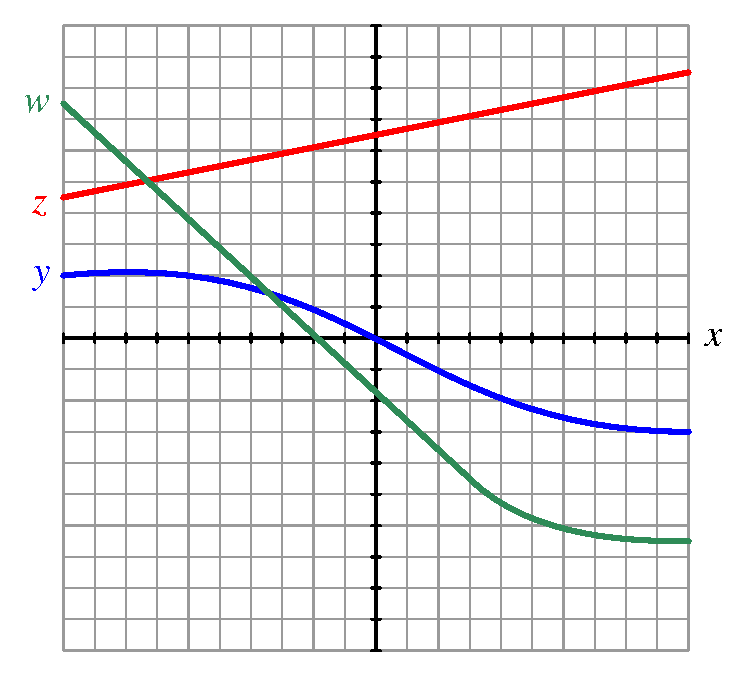
\includegraphics[width=15.5cm]{i01342x01.eps}$$

$$\int_{-5}^{2} (z - y) \> dx$$

Avgjør også om den numeriske verdien av dette integralet er {\it positiv} eller {\it negativ}.

\vskip 20pt \vbox{\hrule \hbox{\strut \vrule{} {\bf Forslag til sokratisk diskusjon} \vrule} \hrule}

\begin{itemize}
\item{} Identifiser noen mulige måleenheter for $z$, $y$ og $x$ som kan passe til dette integralet. Med enhetene du velger, hvilken måleenhet hører da til intervallgrensene $-5$ og 2?
\item{} Utfordre deg selv ved å finne {\it et annet areal} avgrenset av to av funksjonene i dette diagrammet, og skriv deretter et integraluttrykk for dette arealet.
\item{} Utfordre deg selv ved å skrive et vilkårlig integraluttrykk med én funksjon ($y$, $w$ eller $z$), eller differansen mellom {\it to} av disse funksjonene, og velg to start- og sluttpunkter på $x$-aksen (intervallgrenser). Skygg deretter området i diagrammet som representeres av uttrykket.
\end{itemize}

\underbar{file i01342}
%(END_QUESTION)





%(BEGIN_ANSWER)

Dette integralet har en {\it positiv} verdi:

$$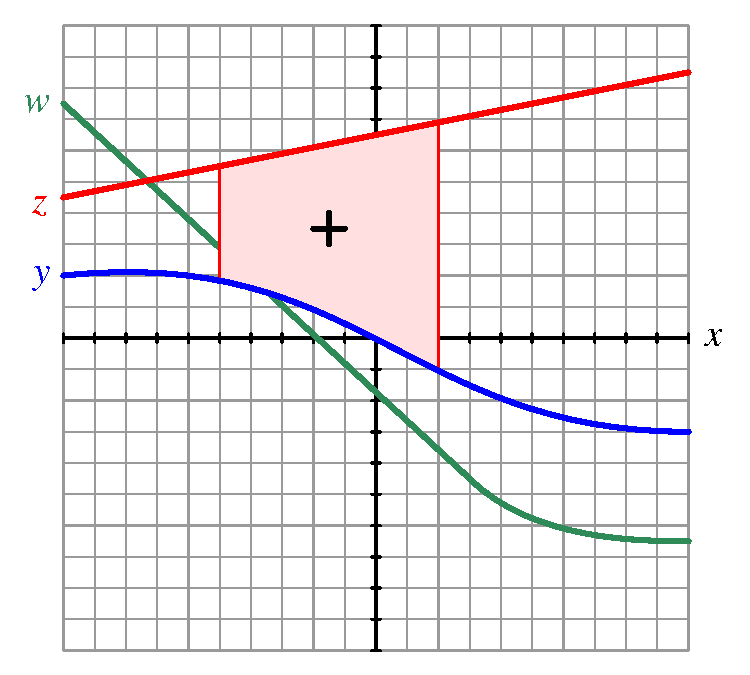
\includegraphics[width=15.5cm]{i01342x02.eps}$$

%(END_ANSWER)





%(BEGIN_NOTES)


%INDEX% Mathematics, calculus: integral (defined in a graphical sense)

%(END_NOTES)

